\section{Inroduction to Graph Theory}

\setcounter{subsection}{3}
\subsection{Definitions, Isomorphism, Degree, Bipartite Graphs}

\begin{xca}
  For the graphs $G_1$, $G_2$, $G_3$, and $H$ in Figure 4.13,
  prove that no two of $G_1$, $G_2$, or $G_3$ are isomorphic.
  Prove that one of them (which?) is isomorphic to $H$ by giving a suitable bijection.
\end{xca}
\begin{sol}
  Isomorphism preserves adjacency, so if a $k$-cycle exists in a graph,
  it must also appear in an isomorphic graph.

  Notice that in $G_1$, to move from one adjacent ``outer'' vertex to another,
  either take the edge connecting them or move down a 4-cycle.

  There is also a 4-cycle in $G_3$.

  In $G_2$, there are no 4-cycles, so $G_1 \not\simeq G_2 \not\simeq G_3$.

  Consider $G_1$ and $G_3$.
  There are exactly two 5-cycles in $G_1$ (outer and inner loops)
  but at least three in $G_2$ (outer, inner, triangle at the bottom).
  We cannot map vertices not in a cycle to a cycle, so $G_1 \not\simeq G_3$.

  Finally, consider $H$.
  Notice that travelling between adjacent outer edges can be accomplished by a 4-cycle.
  This indicates that $H \simeq G_1$ and indeed if we map the inner vertices
  to their vertical reflections, we recover $G_1$.
\end{sol}

\begin{xca}
  A cubic graph is one in which every vertex has degree three.
  Find all the nonisomorphic cubic graphs with 4, 6 and 8 vertices.
\end{xca}
\begin{sol}
  The only cubic graph with 4 vertices is $K_4$
  (every vertex must connect to the other 3, so there is no room to modify).

  In 6 vertices, notice that $K_{3,3}$ is cubic
  (each vertex connecting to the 3 opposite).
  If we construct a triangular prism, this is also cubic.

  In 8 vertices:
  \begin{itemize}
    \item The 3-cube is cubic (for obvious reasons).
          \begin{center}\tikz\graph[clockwise, radius=.75cm] {
            subgraph C_n [n=4] -- subgraph C_n [V={5,6,7,8}] };
          \end{center}
    \item From the 3-cube, we can remove two ``vertical'' edges
          and add diagonals to the top/bottom faces.
          \begin{center}\tikz\graph[clockwise, simple, radius=.75cm] {
            subgraph C_n [n=4] -- subgraph C_n [V={5,6,7,8}],
            4 -!- 8, 2 -!- 6, 4--2, 8--[bend left, dashed]6 };
          \end{center}
    \item If we remove the other two ``verticals'', we get two copies of $K_4$.
    \item From the triangular prism, we can add vertices into two ``vertical'' edges
          or one ``horizontal'' and one ``vertical edge''
          (adding to ``horizontal'' edges gives a cube).
          \begin{center}
            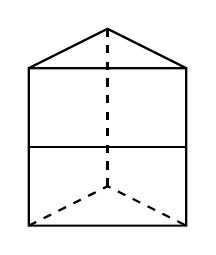
\begin{tikzpicture}
              \draw[dashed,thick] (-1,0) -- (0,0.5) edge (0,2.5) -- (1,0);
              \draw[thick] (-1,0) rectangle (1,2) -- (0,2.5) -- (-1,2);
              \draw[thick] (-1,1) -- (1,1);
            \end{tikzpicture}
            \qquad
            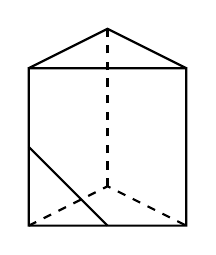
\begin{tikzpicture}
              \draw[dashed,thick] (-1,0) -- (0,0.5) edge (0,2.5) -- (1,0);
              \draw[thick] (-1,0) rectangle (1,2) -- (0,2.5) -- (-1,2);
              \draw[thick] (-1,1) -- (0,0);
            \end{tikzpicture}
          \end{center}
    \item We can take an octagon and pair up vertices:
          \begin{center}
            \tikz\graph{subgraph C_n[n=8, clockwise]; 1--5, 2--6, 3--7, 4--8};
          \end{center}
  \end{itemize}
  which, according to Wikipedia, is exhaustive.
\end{sol}

\begin{xca}
  For the subset graph $S_{n,k}$ defined in Example 4.1.5,
  find the number of vertices and the number of edges.
\end{xca}
\begin{sol}
  There are $\binom{n}{k}$ vertices.
  Each edge takes one of the $k$ elements and replaces it with a different one
  from the $n-k$ others.
  That is, each node has $k(n-k)$ edges.
  By Corollary 4.3.3, this means there are $\frac12k(n-k)\binom{n}{k}$ edges.
\end{sol}

\begin{xca}
  The \term{odd graph} $O_n$ is the graph
  whose vertices are the $n$-subsets of a $(2n+1)$-set,
  two such subsets being adjacent if and only if they are disjoint.
\end{xca}
\begin{enumerate}
  \item Draw $O_1$ and $O_2$.
        \begin{sol}
          The 1-subsets of [3] are $\{1\}$, $\{2\}$, and $\{3\}$
          where they are all disjoint.
          Then, we can draw $O_1$ (omitting curly braces) as
          \begin{center}
            \tikz\graph[clockwise]{ subgraph K_n[n=3] };
          \end{center}
          This is isomorphic to $K_3$.
          The 2-subsets of [5] are 12, 13, 14, 15, 23, 24, 25, 34, 35, and 45.
          We can draw $O_2$ as
          \begin{center}
            \tikz\graph[radius=1.6cm]{ subgraph C_n[V={12,34,15,23,14,25,13,24,35}, clockwise] -!- 45, 15--24, 35--14, 34--25, 12--45--13, 45--23 };
          \end{center}
          as desired.
        \end{sol}
  \item Prove that $O_2$ is isomorphic to the Peterson graph.
        \begin{sol}
          Observe that the layout of $O_2$ is identical to that of $H$ in Figure 4.8.
        \end{sol}
  \item How many vertices and edges does $O_n$ have?
        \begin{sol}
          There are $\binom{2n+1}{n}$ vertices.

          Each each vertex has $\binom{(2n+1)-2}{2} = \binom{2n-1}{2}$ adjacent vertices,
          giving by Corollary 4.3.3 a total of $\frac12\binom{2n+1}{n}\binom{2n-1}{2}$ edges.
        \end{sol}
\end{enumerate}

\begin{xca}
  The \term{line-graph} $L(G)$ of a graph $G$ is the graph
  whose vertex set is $E(G)$ and in which two vertices are adjacent
  if and only if the corresponding edges of $G$ are incident with a common vertex.
\end{xca}
\begin{enumerate}
  \item Find a graph $G$ such that $L(G)$ is isomorphic to $G$.
        \begin{sol}
          Let $G = K_3 = \tikz[baseline=0]\graph[radius=0.5cm,clockwise]{ subgraph K_n[n=3] };$.
          Then, $L(G) = \tikz[baseline=0]\graph[radius=0.5cm,clockwise]{ subgraph K_n[V={12,23,13}] };$
          isomorphic to $G$.
        \end{sol}
  \item Find nonisomorphic graphs $G$, $G'$ such that $L(G)$ is isomorphic to $L(G')$.
        \begin{sol}
          Let $G = K_3$ as above and
          $G' = \tikz[baseline=0]\graph[radius=0.5cm]{ subgraph K_n[clockwise, n=3] -!- 4 };$.

          Since 4 has no edges in $G'$, it does not affect $L(G')$.
          Then, $L(G) = L(G')$ (the same graph as in part (a)).
        \end{sol}
  \item If $G$ is the graph \tikz[baseline=-15pt]\graph[dots nodes]{{1,2}--3[y=-0.5]--4[y=-0.5]--{6,7}};
        find $L(G)$, $L(L(G))$ and $L(L(L(G)))$.
        \begin{sol}
          Calculate $L(G) = \tikz[baseline=-15pt]\graph[dots nodes]{{1,2}--4[y=-0.5]--{6,7}, 1--2, 6--7};$
          and $L(L(G)) = \tikz[baseline=-15pt]\graph[dots nodes]{1[y=-0.5]--{[clique] {2,3}--{4,5}}--6[y=-0.5]};$.

          Finally, $L(L(L(G))) =
            \tikz[baseline=-15pt]\graph[dots nodes, simple]{{1,2}--3[y=-0.5]--{[clique] 4[y=0.5],5[y=0.75,x=-0.35],6[y=1.25,x=0.35],7[y=1.5]}--8[y=-0.5]--{9,10}, 1--2, 9--10, 5-!-6, 4-!-7, 5--1--4, 6--2--7, 4--9--5, 6--10--7};$
        \end{sol}
\end{enumerate}

\begin{xca}
  For integer $n \geq 0$, define the graph $G_n$ as follows:
  $V(G_n)$ is the set of all binary strings of length $n$
  having at most one block of 1's.
  Two vertices are adjacent if they differ in exactly one position.
\end{xca}
\begin{enumerate}
  \item Find $\abs{V(G_n)}$.
        \begin{sol}
          We can map $V(G_n) \bijects S_{n+1,2} \cup \{\varnothing\}$ as follows:
          given $\alpha = 0^i1^j0^k \in V(G_n)$, let $f(\alpha) = \{i,j\}$.
          Then, $f^{-1}(\{\ell,m\}) = 0^\ell 1^m 0^{n-\ell-m}$.
          Map $\varnothing$ to the string $0^n$ with no 1's.
          Notice that for this to work, we define $[n+1] = \{0,\dotsc,n\}$.

          Therefore, $\abs{V(G_n)} = \binom{n+1}{2} + 1 = \frac{1}{2}n(n+1) + 1 = \frac12n^2 + \frac12n + 1$.
        \end{sol}
  \item Make drawings of $G_3$ and $G_4$.
        \begin{sol}
          Construct $V(G_3) = \{000, 100, 010, 001, 110, 011, 111\}$.
          Likewise, construct $V(G_4) = \{0000, 1000, 0100, 0010, 0001, 1100, 0110, 0011, 1110, 0111, 1111\}$.
          Then, notice that differing by exactly one position
          can either add a 1 (swap $0 \to 1$) or remove a 1 ($1 \to 0$).
          Then, we can draw
          \begin{center}
            \tikz\graph[layered layout]{ 000 --[complete bipartite] {100, 010, 001} --[complete bipartite] {110, 011} --[complete bipartite] 111 };
            \qquad
            \tikz\graph[layered layout]{ 0000 --[complete bipartite] {1000, 0100, 0010, 0001} --[complete bipartite] {1100, 0110, 0011} --[complete bipartite] {1110, 0111} --[complete bipartite] 1111 };
          \end{center}
          as desired.
        \end{sol}
  \item Find $\abs{E(G_n)}$.
        \begin{sol}
          Consider the triangle and the $0^n$ separately.
          Between each layer with $i-1$ and $i$ 0's,
          there are $i(i-1)$ edges.
          Then, $\sum_{i=2}^{n} i(i-1) = 2\sum_{i=1}^{n}\binom{i}{2} = 2\binom{n+1}{3}$.
          Finally, there are $n$ edges incident to $0^n$,
          so we have $\abs{E(G_n)} = 2\binom{n+1}{3} + n$.
        \end{sol}
\end{enumerate}

\begin{xca}\end{xca}
\begin{enumerate}
  \item Draw $K_{m,n}$ for all $m$, $n$ such that $1 \leq m \leq n \leq 3$.
        \begin{sol}
          Draw:
          \begin{center}
            \tikz\graph[dots nodes]{ subgraph K_nm[n=1,m=1] };
            \qquad
            \tikz\graph[dots nodes]{ subgraph K_nm[n=1,m=2] };
            \qquad
            \tikz\graph[dots nodes]{ subgraph K_nm[n=1,m=3] };
            \qquad
            \tikz\graph[dots nodes]{ subgraph K_nm[n=2,m=2] };
            \qquad
            \tikz\graph[dots nodes]{ subgraph K_nm[n=2,m=3] };
            \qquad
            \tikz\graph[dots nodes]{ subgraph K_nm[n=3,m=3] };
          \end{center}
          as desired.
        \end{sol}
  \item How many vertices does $K_{m,n}$ have?
        \begin{sol}
          There are $\abs{V(K_{m,n})} = m + n$ vertices.
        \end{sol}
  \item Let $K$ be a complete bipartite graph on $p$ vertices.
        Prove that $K$ has at most $\floor{p^2/4}$ edges.
        \begin{sol}
          Suppose $K \simeq K_{m,n}$.
          Then, there are $\abs{E(K)} = \abs{E(K_{m,n})} = m \times n$ edges
          to connect each of the $m$ left vertices to $n$ right vertices.

          \WLOG, suppose $m \leq n$.
          By high school algebra, $\abs{E(K)}$ is maximized when $m = n$.

          If $p$ is even, let $m = n = \frac{p}{2}$.
          Then, $\abs{E(K)} \leq \frac{p^2}{4}$.

          If $p = 2k+1$ is odd, let $m = k = \floor{\frac{p}{2}}$ and $n = k+1 = \floor{\frac{p}{2}}+1$.
          Notice that $\floor{\frac{p^2}{4}} = \frac{4k^2+4k+1}{4} = k^2+k$.
          Then, $\abs{E(K)} \leq mn = k^2 + k = \floor{\frac{p^2}{4}}$,

          Therefore, $K$ has at most $\floor{\frac{p^2}{4}}$ edges.
        \end{sol}
  \item Let $G$ be a bipartite graph on $p$ vertices.
        Prove that $G$ has at most $\floor{p^2/4}$ edges.
        \begin{sol}
          Since $G$ is bipartite, all edges cross the bipartition
          $(A,B)$ where $\abs{A} = m$ and $\abs{B} = n$.
          That is, all edges exist in $K_{m,n}$.

          Thus, $G$ is a subgraph of $K_{m,n}$
          and by (c), $\abs{E(G)} \leq \abs{E(K_{m,n})} \leq \floor{\frac{p^2}{4}}$, as desired.
        \end{sol}
  \item Let $G$ be a $k$-regular bipartite graph with bipartition $(X,Y)$.
        Prove that $\abs{X} = \abs{Y}$ if $k > 0$.
        Is this still valid when $k=0$?
        \begin{prf}
          Let $k \geq 1$ and suppose $\abs{X} \neq \abs{Y}$.

          Then, notice that since $G$ is bipartite, by definition,
          the edges incident to $X$ are the edges incident to $Y$,
          i.e., $\abs{\delta(X)} = \abs{\delta(Y)}$.
          But each of $X$ (resp.\ $Y$) consist of $\abs{X}$
          vertices of $k$ degree going to vertices in $Y$,
          so $\abs{\delta(X)} = k\abs{X} = k\abs{Y} = \abs{\delta(Y)}$.

          But $\abs{X} \neq \abs{Y}$, implying $k = 0$. Contradiction.

          This is not valid when $k=0$.
          Notice that if $V(G) = \{1\}$, $E(G) = \varnothing$,
          $X = \{1\}$, and $Y = \varnothing$,
          we have a 0-regular bipartite graph with bipartition $(X,Y)$
          and $\abs{X} \neq \abs{Y}$.
        \end{prf}
\end{enumerate}

\begin{xca}
  The \term{complement} of a graph $G$, denoted $\bar G$,
  is the graph with $V(\bar G) = V(G)$
  and the edge $uv \in E(\bar G)$ if and only if $uv \not\in E(G)$.
\end{xca}
\begin{enumerate}
  \item Let $G$ have vertices 1, 2, 3, 4 and edges 12, 23, 34, 14. Draw $\bar G$.
        \begin{sol}
          Note that $E(\bar G) = \{13,24\}$ (with $E(G)$ in dashes):
          \begin{center}
            \tikz\graph[simple necklace layout]{1,2,3,4; 1--3; 2--4; {[edges=dashed] 1--2--3--4--1, 3--4}};
          \end{center}
          as desired.
        \end{sol}
  \item Find a 5-vertex graph that is isomorphic to its complement.
        \begin{sol}
          Consider the 5-cycle $C_5$ and its complement (dashed) $\bar C_5$:
          \begin{center}
            \tikz\graph{subgraph C_n[n=5, clockwise]; {[edges=dashed] 1--3--5--2--4--1}};
          \end{center}
          and notice that the complement is the cycle $\{1,3,5,2,4\}$.
        \end{sol}
  \item Prove that no 6-vertex graph is isomorphic to its complement.
        \begin{prf}
          Notice that for a graph $G$, we have $E(G) \cup E(\bar G)$
          is a disjoint union of the set of subsets of $V(G)$ with size 2.

          Notice that for a 6-vertex graph, there are $\binom{6}{2} = 15$
          subsets of $V(G)$ with size 2.
          These cannot be partitioned into $\abs{E(G)} = \abs{E(\bar G)}$
          because 15 is odd.
        \end{prf}
  \item Let $G_1$ and $G_2$ be two graphs.
        Prove that $G_1$ is isomorphic to $G_2$
        if and only if $\bar G_1$ is isomorphic to $\bar G_2$.
        \begin{prf}
          Suppose $G_1 \simeq G_2$.
          Then, there exists an isomorphism $\phi : V(G_1) \to V(G_2)$
          such that $uv \in E(G_1) \iff \phi(u)\phi(v) \in E(G_2)$.
          It follows that
          \[ uv \in E(\bar G_1) \iff uv \not\in E(G_1) \iff \phi(u)\phi(v) \not\in E(G_2) \iff \phi(u)\phi(v) \in E(\bar G_2) \]
          so $\phi$ is also an isomorphism between $\bar G_1$ and $\bar G_2$.

          Finally, since $\bar{\bar G} = G$ (because $E(G)$ and $E(\bar G)$ are set complements),
          this goes in both directions.
        \end{prf}
  \item Find all 2-regular non-isomorphic graphs on 6 vertices
        (prove that these are the only ones).
        \begin{prf}
          Notice that a 2-regular component is a cycle.
          The smallest cycle is the 3-cycle,
          so we can either have two 3-cycles or one 6-cycle.
        \end{prf}
  \item Prove that there are only two 3-regular non-isomorphic graphs on 6 vertices.
        \begin{prf}
          Let $G$ be such a graph.
          For each vertex, there are three incident edges.
          The other two potential edges lie in the complement.
          Therefore, $\bar G$ is a 2-regular graph on 6 vertices.
          By (d), the complement preserves isomorphism.
          By (e), there are only two classes of 2-regular isomorphic graphs on 6 vertices.
          Therefore, there must be only two 3-regular non-isomorphic graphs on 6 vertices.
        \end{prf}
\end{enumerate}

\begin{xca}
  Make drawings of the 15 non-isomorphic graphs having six vertices and six edges,
  such that every vertex has degree at least one.
\end{xca}

\begin{xca}
  Are the graphs in Figure 4.14 isomorphic? Justify your answer.
\end{xca}

\begin{xca}\label{xca:prime}
  For $n$ a positive integer, define the \term{prime graph} $B_n$
  to be the graph with vertex set $\{1,2,\dotsc,n\}$,
  where $\{u,v\}$ is an edge if and only if $u + v$ is a prime number.
  Prove that $B_n$ is bipartite.
\end{xca}
\begin{prf}
  Notice that for $u+v > 2$ to be prime, it must be odd
  (since we cannot have a $\{1,1\}$ loop to make 2).
  Therefore, exactly one of $u$ and $v$ must be odd.
  It follows that if we partition $V(B_n) = [n]$
  into $X = \{ i \in [n] : i \bmod 2 = 0 \}$ and $Y = \{ i \in [n] : i \bmod 2 = 1 \}$,
  we have a bipartition of $B_n$.
\end{prf}

\subsection{How to Specify a Graph}

Not covered in Fall 2022 offering.

\subsection{Paths and Cycles}
\begin{xca}\label{xca:deg-path}
  Let $G$ be a graph with minimum degree $k$, where $k \geq 2$.
  Prove that:
\end{xca}
\begin{enumerate}
  \item $G$ contains a path of length at least $k$
        \begin{prf}
          Proceed by induction on $k$.
          Let $v \in V(G)$ be a vertex.

          If $k = 0$, then notice that $v$ is a path of length 0.

          If $k = 1$, then $v$ must have a neighbour $u$.
          Then, $v,u$ is a path of length 1.

          For $k \geq 2$, since $k > k-1$, suppose
          there exists a path $P = v_0,\dotsc,v_{k-1}$ of length $k-1$.
          Since $v_{k-1}$ has degree at least $k$, $\abs{N_G(v_{k-1})} \geq k$,
          so $\abs{N_G(v_{k-1}) \setminus \{v_0,\dotsc,v_{k-2}\}} \geq 1$.
          Let $v_k \in N_G(v_{k-1}) \setminus \{v_0,\dotsc,v_{k-2}\}$
          and notice that $P + v_k$ is a path of length $k$.
        \end{prf}
  \item $G$ contains a cycle of length at least $k+1$
        \begin{prf}
          By part (a), a path of length at least $k$ exists in $G$.
          Let $P = v_0,\dotsc,v_k,\dotsc,v_\ell$ be the longest such path.
          Then, as above, notice that $\abs{N_G(v_\ell) \setminus \{v_{\ell-k},\dotsc,v_{\ell-1}\}} \geq 1$.
          Select any $x \in N_G(v_\ell) \setminus \{v_{\ell-k+1},\dotsc,v_{\ell-1}\}$.
          If $x \not\in P$, then $P' = P + x$ is a longer path.
          Otherwise, $x = v_i$ for $0 \leq i \leq \ell-k$.

          The cycle $v_i,\dotsc,v_\ell$ has length at least $k+1$.
        \end{prf}
\end{enumerate}

\setcounter{xca}{3} % Skip adjacency matrix questions

\begin{xca}
  Let $G$ be the graph whose set of vertices is the set of all
  ``lower 48'' states of the United States, plus Washington, DC,
  with two vertices being adjacent if they share a boundary.
  Let $H$ be the subgraph of $G$ whose vertices are those of $G$
  whose first letter is one of W, O, M, A, N,
  and whose edges are the edges of G whose ends have this property.
  Find a path in $H$ from Washington to Washington, DC.
\end{xca}
\begin{sol}
  Consult a map and get WA, OR, NV, AZ, NM, OK, MO, NB, WY, MT, ND, MN, WI, MI, OH, WV, MD, DC.
\end{sol}

\begin{xca}
  Consider the word graph $W_n$ defined in Example 4.1.2.\footnote{
    $V(W_n)$ is the set of English words of length $n$
    with adjacency if they differ by exactly one letter.}
\end{xca}
\begin{enumerate}
  \item Find a cycle through \emph{math} in $W_4$.
        \begin{sol}
          (\emph{math}, \emph{meth}, \emph{mete}, \emph{mate}, \emph{math})
          is a cycle in $W_4$.
        \end{sol}
  \item Find a path from \emph{pink} to \emph{blue} in $W_4$.
        \begin{sol}
          (\emph{pink}, \emph{tink}, \emph{tank}, \emph{tans}, \emph{tens}, \emph{fens}, \emph{feus}, \emph{flus}, \emph{flue}, \emph{blue})
          using words in Merriam--Webster.
        \end{sol}
\end{enumerate}

\begin{xca}
  For $n \geq 2$, prove that the $n$-cube contains a Hamilton cycle.
\end{xca}
\begin{prf}
  Let $G_n$ denote the $n$-cube. Proceed by induction on $n$.

  Notice that for $n = 2$, $(00,01,11,10,00)$ is a Hamilton cycle.

  Let $n \geq 3$.
  Partition $V(n) = V_0 \cup V_1$ based on the first digit in the binary string.
  Now, the subgraphs induced by $V_0$ and $V_1$ are isomorphic to $G_{n-1}$
  under the isomorphism $f_b : G_{n-1} \to V_b : \alpha \mapsto b\alpha$
  and inverse $f^{-1}_b : V_b \to G_{n-1} : b_1\cdots b_n \to b_2 \cdots b_n$.

  Assume $G_{n-1}$ has a Hamilton cycle.
  \WLOG, suppose that it begins at $0^{n-1}$ and ends at $0^{n-2}1$,
  so that $V_0$ has a Hamilton cycle $(00^{n-2}0, \dotsc, 00^{n-2}1)$
  and $V_1$ has a Hamilton cycle $(10^{n-2}0, \dotsc, 10^{n-2}1)$.

  Then, $(00^{n-2}0, \dotsc, 00^{n-2}0, 10^{n-2}0, \dotsc, 10^{n-2}1, 00^{n-2}1)$
  is a Hamilton cycle for $G_n$.
\end{prf}

\begin{xca}
  Prove that the complete bipartite graph $K_{m,n}$ has a Hamilton cycle
  if and only if $m = n$ and $m > 1$.
\end{xca}
\begin{prf}
  Suppose $m = n$ and $m > 1$.
  Then, $(s_1,t_1,s_2,t_2,\dotsc,s_m,t_n)$ is a Hamilton cycle.

  Conversely, assume \Wlog that $m \leq n$ and that there is a Hamilton cycle.

  When $m = 0$, there are no edges and no Hamilton cycle.
  For $m = 1$, trace the Hamilton cycle starting at $s_1$.
  First $N(s_1) = \{t_i\}$, so the next vertex must be $t_k$ for some $k$.
  However, $N(t_k) = \{s_1\}$ and we cannot continue because $s_1t_k$ is already in the cycle.

  Otherwise, suppose $m \neq n$ and $1 < m < n$.
  Every edge is $s_i t_j$, so the cycle goes $s_{a_1},t_{b_1},s_{a_2},t_{b_2},\dotsc$.
  At $t_{b_m}$, we have visited $m$ vertices $s_i$, i.e., all of them.
  Therefore, the cycle must end here and return to $s_{a_1}$.
  However, there are vertices $t_{b_{m+1}},\dotsc,t_{b_n}$ which are not in the cycle.
  That is, the cycle is not a Hamilton cycle.

  Therefore, there is a Hamilton cycle if and only if $m = n$ and $m > 1$.
\end{prf}

\begin{xca}\label{xca:oddcycle}
  Show that if there is a closed walk of odd length in the graph $G$,
  then $G$ contains an odd cycle
  (that is, $G$ has a subgraph which is a cycle on an odd number of vertices).
\end{xca}
\begin{prf}
  Suppose that $W = v_1,\dotsc,v_n,v_1$
  is the shortest closed walk of odd length that exists in $G$ (i.e., $n$ is odd).

  Induct on the number of such vertices in $W$ that appear multiple times.

  If $W$ is a path, i.e., there are no such vertices, $W$ is a cycle and we are done.

  Otherwise, there exists $i$ and $j$ such that $v_i = v_j$.
  Then, the edges in $W$ can be partitioned into two closed walks
  $W_1 = v_1,\dotsc,v_{i-1},v_i,v_{j+1},\dotsc,v_1$ and $W_2 = v_i,v_{i+1},\dotsc,v_{j-1},v_i$.
  Since $W$ has an odd number of edges and $E(W_1) \cup E(W_2)$ partition $E(W)$,
  exactly one of $W_1$ and $W_2$ has an odd number of edges.
  By the inductive hypothesis, since that walk necessarily has fewer duplicates,
  there exists an odd cycle in that walk.

  Therefore, there exists an odd cycle in $G$.
\end{prf}

\begin{xca}
  A \term{diagonal} of a cycle in a graph is an edge that joins vertices
  that are not consecutive in the cycle.
\end{xca}
\begin{enumerate}
  \item Prove that a shortest cycle has no diagonal.
        \begin{prf}
          Let $C = v_1,\dotsc,v_k,v_1$ be a shortest cycle.
          Suppose a diagonal $v_iv_j$, $i < j$, $j \neq i + 1$ exists.
          Then, $v_1,\dotsc,v_i,v_j,\dotsc,v_k,v_1$
          is a shorter cycle. Contradiction.
        \end{prf}
  \item Prove that a shortest odd cycle has no diagonal.
        \begin{prf}
          Let $C = v_1,\dotsc,v_k,v_1$ be a shortest odd cycle, i.e., $k$ is odd.
          Suppose a diagonal $v_iv_j$, $i < j$, $j \neq i + 1$ exists.
          Then, as in \cref{xca:oddcycle}, we can create two cycles
          $C_1 = v_1,\dotsc,v_i,v_j,\dotsc,v_k,v_1$
          and $C_2 = v_i,\dotsc,v_j,v_i$.

          Since $V(C_1) \cap V(C_2) = \{v_i,v_j\}$,
          we have $\abs{V(C)} = \abs{V(C_1)} + \abs{V(C_2)} - 2$.
          That is, $1 \equiv \abs{V(C_1)} + \abs{V(C_2)} \pmod{2}$.
          Then, either $C_1$ or $C_2$ must be a shorter odd cycle.
          Contradiction.
        \end{prf}
  \item Give an example of a graph in which a shortest even cycle has a diagonal.
        \begin{sol}
          The minimal example \tikz[baseline=-3pt]\graph[dots nodes, radius=0.5cm]{ subgraph C_n[n=4, clockwise], 1--3 };.
        \end{sol}
\end{enumerate}

\begin{xca}\end{xca}
\begin{enumerate}
  \item Prove that a $k$-regular graph of girth 4 has at least $2k$ vertices ($k \geq 2$).
  \item For $k = 2,3$, find a $k$-regular graph of girth 4 with precisely $2k$ vertices.
        Generalize these examples to find one for each $k \geq 2$.
  \item Prove that a $k$-regular graph of girth 5 has at least $k^2+1$ vertices ($k \geq 2$).
  \item Prove that a $k$-regular graph of girth $2t$, where $t \geq 2$,
        has at least $\frac{2(k-1)^t-2}{k-2}$ vertices.
  \item Prove that a $k$-regular graph of girth $2t+1$, where $t \geq 2$,
        has at least $\frac{k(k-1)^t-2}{k-2}$ vertices.
  \item For $k = 2,3$, give an example of a $k$-regular graph of girth 5
        with exactly $k^2+1$ vertices.
\end{enumerate}

\setcounter{subsection}{9}
\subsection{Equivalence Relations, Connectedness, Eulerian Circuits, Bridges}

\begin{xca}
  Prove that the prime graph $B_n$ defined in \Cref{xca:prime} is connected for every $n$.
  You may use without proof the following fact:
  For every integer $k \geq 2$,
  there is a prime number $r$ such that $k < r < 2k$.
\end{xca}
\begin{prf}
  Proceed by induction on $n$.
  Clearly, $B_1$ is connected with a single vertex.

  Let $n \geq 2$. We may assume that $B_{n-1} = B_n - n$ is connected.

  There exists a prime number $r$ such that $n < r < 2n$.
  That is, $r = n + m$ for $1 \leq m \leq n-1$.
  Since $m \in \{1,\dotsc,n-1\} \subseteq [n] = V(B_n)$,
  the edge $mn$ exists in $B_n$.
  For any $k \in V(B_n) \setminus \{n\} = V(B_{n-1})$,
  since $B_{n-1}$ is connected, there exists a $k,m$-path.
  Adjoining $mn$, there exists a $k,n$-path in $B_n$.

  Therefore, by Theorem 4.8.2, $B_n$ is connected.
\end{prf}

\begin{xca}
  Prove that if $G$ is connected,
  any two longest paths have a vertex in common.
\end{xca}
\begin{prf}
  Let $P_1$ be a $s,t$-path and $P_2$ be a $u,v$-path in $G$
  such that both $P_1$ and $P_2$ are longest paths in $G$ with length $k$.

  Then, suppose that $V(P_1) \cap V(P_2) = \varnothing$.

  Since $G$ is connected, there exists a $t,u$-path $P_3$ in $G$.
  Consider the walk $W = P_1P_3P_2$.
  By the process in the proof in Theorem 4.6.2,
  there exists a $s,v$-path $P$ using all the non-overlapping
  vertices in $P_1$ and $P_2$ (but only some of $P_3$).
  That is, $P$ has length at least $2k$, meaning that $P_1$ and $P_2$ are not longest paths.

  Therefore, by contradiction, $P_1$ and $P_2$ must share a vertex.
\end{prf}

\begin{xca}
  Which graphs, with at least one edge,
  have the property that every edge is a bridge?
\end{xca}
\begin{sol}
  By Theorem 4.10.3, an edge is a bridge if and only if it is not contained in a cycle.
  Therefore, every edge is a bridge if and only if the graph contains no cycles.
  That is, the graph is a forest.
\end{sol}

\begin{xca}
  If every vertex of a graph $H$ with $p$ vertices has degree at least $\frac{p}{5}$,
  prove that $H$ cannot have more than 4 components.
\end{xca}
\begin{prf}
  Let $v \in V(H)$. Since $\deg v \geq \frac{p}{5}$,
  its component has size at least $\frac{p}{5} + 1$.

  This applies to all components, so if there are $k$ components,
  $p \geq k(\frac{p}{5}+1)$, that is, $k \leq \frac{p}{\frac{p}{5}+1} < \frac{p}{p/5} = 5$.
  Therefore, there are at most 4 components.
\end{prf}

\begin{xca}
  If an edge $e$ is not a bridge of a connected graph $G$,
  prove that $e$ is an edge of some cycle.
\end{xca}
\begin{prf}
  If $e = uv \in E(G)$ is not a bridge, then $G - e$ remains connected.
  But that means there is a $u,v$-path $P$ in $G - e$.
  Then, $P + e$ is a cycle in $G$ containing $e$.
\end{prf}

\begin{xca}
  Prove that a 4-regular graph has no bridge.
\end{xca}
\begin{prf}
  Consider an edge $e = uv$ in a 4-regular component $G$.
  Then, by the proof of \Cref{xca:deg-path}, $e$ lies in a 5-cycle.
  Since $e$ lies in a cycle, it is not a bridge by Theorem 4.10.3.
\end{prf}

\begin{xca}\label{xca:4107}
  Let $A_n$ be the graph whose vertices are the $\{0,1\}$-strings of length $n \geq 2$,
  and edges are between strings that differ in exactly two positions.
\end{xca}
\begin{enumerate}
  \item How many edges does $A_n$ have?
        \begin{sol}
          Since each of the $2^n$ strings have $\binom{n}{2}$ neighbours
          (must pick two positions to change),
          we have $\abs{E(A_n)} = \binom{n}{2}2^{n-1}$ by the Handshaking Lemma.
        \end{sol}
  \item Is $A_n$ bipartite for any $n \geq 2$?
        \begin{sol}
          When $n = 2$, $V(A_2) = \{00,01,10,11\}$
          and $E(A_2) = \{\{00,11\},\{01,10\}\}$
          which is bipartite with bipartition $(X,Y) = (\{00,11\},\{01,10\})$.

          For $n \geq 3$, there exists an odd cycle
          $(0000^{n-3}, 0110^{n-3}, 1100^{n-3}, 0000^{n-3})$.
          Therefore, by Theorem 5.3.2, $A_n$ is not bipartite.
        \end{sol}
  \item How many components does $A_n$ have?
        \begin{sol}
          Claim: there are two components.

          Divide the elements of $V(A_n)$ by parity.
          Notice that changing exactly two positions either sends
          two 0's to two 1's, two 1's to two 0's, or one of each (cancelling).
          These do not change the parity.
          Therefore, no path exists between any string of even and odd parity.

          Now, consider two strings with the same parity.
          Then, they differ by an even number of positions.
          By changing two at a time, there exists a path between them.

          Therefore, there are exactly two components of $A_n$.
        \end{sol}
\end{enumerate}

\begin{xca}
  Let $B_n$ be the graph whose vertices are the $\{0,1\}$-strings of length $n \geq 2$,
  and edges are between strings that differ in exactly two consecutive positions.
\end{xca}
\begin{enumerate}
  \item How many edges does $B_n$ have?
        \begin{sol}
          The neighbours of a string can differ in the positions starting at $1,\dotsc,n-1$.
          That is, the degree of every vertex is $n-1$.
          By the Handshaking Lemma, since $\abs{V(B_n)} = 2^n$,
          $\abs{E(B_n)} = (n-1)2^{n-1}$.
        \end{sol}
  \item How many components does $B_n$ have?
        \begin{sol}
          There are at least two components by \Cref{xca:4107}.

          Consider two strings with even parity.
          Follow a path sending each instance of 01 to 10.
          This will give a string of the form $1^{2k}0^{n-2k}$.
          Then, there is clearly a path to $0^n$.
          Therefore, all the even parity strings form a single component by Theorem 4.8.2.

          Likewise, for odd parity strings, there is always a path to $10^{n-1}$
          and they form a single component by Theorem 4.8.2.

          Therefore, there are exactly two components of $B_n$.
        \end{sol}
\end{enumerate}

\begin{xca}
  Let $G$ be a graph in which exactly two of the vertices $u$ and $v$ have odd degree.
  Prove that $G$ contains a path from $u$ to $v$.
\end{xca}
\begin{prf}
  Suppose there is not a $u,v$-path.
  That is, $u$ and $v$ lie in different components.
  Then, every $w \in [u]$, $w \neq u$ has even degree.
  By the Handshaking Lemma, 
  \[ 
    0 \equiv 2\abs{E(G)}
    \equiv \sum_{w \in [u]} \deg(w)
    \equiv \deg(v) + \sum_{\substack{w \in [u] \\ w \neq v}}\deg(w)
    \equiv 1 + \sum_{\substack{w \in [u]\\w \neq v}}0 \equiv 1 \pmod{2}
  \]
  which is a contradiction. Therefore, $v \in [u]$ and there must exist a $u,v$-path.
\end{prf}
